\documentclass[a4paper,12pt]{report}

% Page layout
\usepackage[left=2.5cm,right=2.5cm,top=2.5cm,bottom=2.5cm]{geometry}

% Font and text
\usepackage[afrikaans,english]{babel}
\usepackage{microtype}
\usepackage{setspace}
\usepackage{lmodern}
\usepackage{siunitx}
\usepackage{ mathrsfs }
\newcommand{\myemph}[1]{{\sffamily\bfseries#1}}
\sloppy
\onehalfspacing

% Headings
\usepackage[raggedright,sf,bf]{titlesec}
\usepackage[margin=\the\parindent,small,bf,sf]{caption}
\titlelabel{\thetitle.\ }
\titleformat{\chapter}[display]{\huge\bfseries\sffamily}{\chaptertitlename\ \thechapter}{15pt}{\Huge \raggedright}
\titlespacing*{\chapter}{0pt}{0pt}{40pt}  % remove spacing before chapter headings
\makeatletter
\let\originall@chapter\l@chapter
\def\l@chapter#1#2{\originall@chapter{{\sffamily #1}}{#2}}
\makeatother

% Alternative headings using small-caps (comment out the top section)
\usepackage[raggedright,bf]{titlesec}
\usepackage[margin=\the\parindent,small,bf]{caption}
\titlelabel{\thetitle.\ }
\titleformat{\chapter}[display]{\huge\scshape}{\chaptertitlename\ \thechapter}{15pt}{\Huge \raggedright}
\titlespacing*{\chapter}{0pt}{0pt}{40pt}  % remove spacing before chapter headings

% Table of contents
\let \savenumberline \numberline
\def \numberline#1{\savenumberline{#1.}}

% Figures
\usepackage{graphicx}
\usepackage{pdfpages}
\usepackage{subcaption}
\setlength{\abovecaptionskip}{7.5pt}  % spacing above and below captions
\newcommand*{\WaterMark}[2][0.2\paperwidth]{\AddToShipoutPicture*{\AtTextCenter{\parbox[c]{0pt}{\makebox[0pt][c]{\includegraphics[width=#1]{#2}}}}}}

% Mathematics
\usepackage[cmex10]{amsmath}
\usepackage{amssymb}
\usepackage{cancel}
\DeclareMathOperator*{\argmax}{arg\,max}
\newcommand{\T}{^\top}
\newcommand{\tr}{\textrm{tr}}
\renewcommand{\vec}[1]{\boldsymbol{\mathbf{#1}}}
\newcommand{\defeq}{\triangleq}

% Tables
\usepackage{booktabs}
\usepackage{tabularx}
\usepackage{multirow}
\newcommand{\mytable}{
    \centering
    \small
    \renewcommand{\arraystretch}{1.2}
    }
\renewcommand{\tabularxcolumn}[1]{m{#1}}
\newcolumntype{C}{>{\centering\arraybackslash}X}
\newcolumntype{L}{>{\raggedright\arraybackslash}X}

% Header and footer
\usepackage{fancyhdr}
\pagestyle{fancy}
\fancyhf{}
\renewcommand{\sectionmark}[1]{\markright{\normalsize \thesection.\ #1}}
\fancyhead[C]{\nouppercase{\textit{\rightmark}}}
\fancyhead[RO]{\thepage}
 \fancyhead[LE]{\thepage}  % double-sided printing
\fancyfoot{}
\setlength\headheight{14.5pt}
\renewcommand{\headrulewidth}{0pt}
\fancypagestyle{plain}{\fancyhead{}
                       \renewcommand{\headrulewidth}{0pt}
                       \fancyfoot[C]{\thepage}}

% Pseudo-code
\usepackage{algorithm}  % should go before \usepackage{hyperref}

% Table of contents and hyperlinks
\usepackage{hyperref}
\hypersetup{colorlinks=true,linktoc=all,citecolor=black,linkcolor=black}
\usepackage[nottoc]{tocbibind}

% Pseudo-code
\usepackage{algpseudocode}  % should go after \usepackage{hyperref}
\renewcommand{\thealgorithm}{\arabic{chapter}.\arabic{algorithm}} 
\captionsetup[algorithm]{labelfont={bf,sf},font=small,labelsep=colon}

% Bibliography
\usepackage{cite}  % automatically reorder inline citations
\bibliographystyle{IEEEtran}

% Fix titlesec issue
\usepackage{etoolbox}
\makeatletter
\patchcmd{\ttlh@hang}{\parindent\z@}{\parindent\z@\leavevmode}{}{}
\patchcmd{\ttlh@hang}{\noindent}{}{}{}
\makeatother

% Misc Packages & Commands
\usepackage{enumitem}
\usepackage{url} % Hopefully no line breaks on my urls...
\newcommand\numberthis{\addtocounter{equation}{1}\tag{\theequation}}


\begin{document}

% Front matter
\graphicspath{{frontmatter/fig/}}
\pagenumbering{Alph}

\begin{titlepage}
	\begin{center}
		
		
\includegraphics[width=10cm]{USlogo-top}
		
		\vfill
		
		{\sffamily \bfseries \huge A Critical Analysis of Design Flaws in the Death Star \par}
%		{\scshape \huge A Critical Analysis of Design Flaws in the Death Star \par}
		
		\vfill
		
		{\large {\Large Luke Skywalker} \\ 99652154 \par}
		
		\vfill
		
		\vfill
		
		{Report submitted in partial fulfilment of the requirements of the module \\
			Project (E) 448 for the degree Baccalaureus in Engineering in the Department of
			Electrical and Electronic Engineering at Stellenbosch University. \par}
		
		\vfill
		
		{\large {Supervisor}: Dr O.\ W.\ Kenobi} %\\
		% Department of Electrical and Electronic Engineering \par}
		
		\vfill
		
		{\Large October 2099}
	\end{center}
\end{titlepage}

%\graphicspath{{frontmatter/fig/}}
\pagenumbering{Alph}

\begin{titlepage}
	\begin{center}
		
		%
\includegraphics[width=10cm]{USlogo-top}
		
		\WaterMark{UScrest-WM}
		
		~\vspace{4.5em}
		
		{\sffamily \bfseries \huge A Critical Analysis of Design Flaws in the Death Star \par}
%		{\scshape \huge A Critical Analysis of Design Flaws in the Death Star \par}		
		
		\vspace{7em}
		
		{\large {\Large  Luke Skywalker} \\ 99652154 \par}
		
		\vspace{8em}
		
		{\large Thesis presented in partial fulfilment of the requirements for the degree of \\ Master of Engineering (Electronic) in the Faculty of Engineering at Stellenbosch University. \par}
		
		\vfill
		
		{\large {Supervisor}: Dr O.\ W.\ Kenobi\\
		Department of Electrical and Electronic Engineering \par}
		
		%\vfill
		\vspace{10em}
		
		{\Large October 2099}
	\end{center}
\end{titlepage}

\pagenumbering{roman}
\chapter*{Acknowledgements}
% \addcontentsline{toc}{chapter}{Acknowledgements}
\makeatletter\@mkboth{}{Acknowledgements}\makeatother

<TODO: Do Really need this?>

I would like to thank my dog, Muffin. I also would like to thank the inventor of the incubator; without him/her, I would not be here. Finally, I would like to thank Dr Herman Kamper for this amazing report template.

%\chapter*{Declaration}
\newpage
\thispagestyle{plain}
\addcontentsline{toc}{chapter}{Declaration}
\makeatletter\@mkboth{}{Declaration}\makeatother

\centerline{
\includegraphics[width=8cm]{USlogo-top}}
\vspace*{-10pt}

\section*{\centering Plagiaatverklaring / \textit{Plagiarism Declaration}}

\vspace*{5pt}

\begin{enumerate}
    \item Plagiaat is die oorneem en gebruik van die idees, materiaal en ander intellektuele eiendom van ander persone asof dit jou eie werk is.\\
    \textit{Plagiarism is the use of ideas, material and other intellectual property of another's work
        and to present is as my own.}
    
    \item Ek erken dat die pleeg van plagiaat 'n strafbare oortreding is aangesien dit 'n vorm van diefstal is.\\
    \textit{I agree that plagiarism is a punishable offence because it constitutes theft.}
    
    \item Ek verstaan ook dat direkte vertalings plagiaat is. \\
    \textit{I also understand that direct translations are plagiarism.}
    
    \item Dienooreenkomstig is alle aanhalings en bydraes vanuit enige bron (ingesluit die internet) volledig verwys (erken). Ek erken dat die woordelikse aanhaal van teks sonder aanhalingstekens (selfs al word die bron volledig erken) plagiaat is. \\
    \textit{Accordingly all quotations and contributions from any source whatsoever (including the internet) have been cited fully. I understand that the reproduction of text without quotation marks (even when the source is cited) is plagiarism}
    
    \item Ek verklaar dat die werk in hierdie skryfstuk vervat, behalwe waar anders aangedui, my eie oorspronklike werk is en dat ek dit nie vantevore in die geheel of gedeeltelik ingehandig het vir bepunting in hierdie module/werkstuk of 'n ander module/werkstuk~nie. \\
    \textit{I declare that the work contained in this assignment, except where otherwise stated, is my original work and that I have not previously (in its entirety or in part) submitted it for grading in this module/assignment or another module/assignment.}
\end{enumerate}

\vfill

\noindent \begin{tabularx}{1.0\linewidth}{|L|L|}
    \hline
    \vspace{1cm} {Studentenommer / \textit{Student number}} & \vspace{1cm} {Handtekening / \textit{Signature}} \\
    \hline
    \vspace{1cm} {Voorletters en van / \textit{Initials and surname}} & \vspace{1cm} {Datum / \textit{Date}} \\
    \hline
\end{tabularx}

\vspace{15pt}

% The old declaration

%I, the undersigned, hereby declare that the work contained in this report is my own original work unless otherwise stated.
%
%% Afrikaans:
%% Hiermee verklaar ek, die ondergetekende, dat die werk in hierdie verslag vervat my eie oorspronklike werk is, tensy anders vermeld.
%
%\vspace{2.5cm}
%
%\begin{table}[h]
%\begin{tabular}{@{}p{2.5cm}p{5cm}}
%    Signature: & \dotfill \\
%    & \multicolumn{1}{c}{Obi-Wan Kenobi} \\
%    ~\vspace{1cm} \\
%    Date: & \dotfill \\
%\end{tabular}
%\end{table}
%
%\vfill
%
%\begin{center}
%    Copyright \textcopyright\ 2099 Stellenbosch University \\
%    All rights reserved
%\end{center}


\chapter*{Abstract}
\addcontentsline{toc}{chapter}{Abstract}
\makeatletter\@mkboth{}{Abstract}\makeatother

\subsubsection*{English}

The English abstract.

\selectlanguage{afrikaans}

\subsubsection*{Afrikaans}

Die Afrikaanse uittreksel.

\selectlanguage{english}
\tableofcontents
\listoffigures
\listoftables
\chapter*{Nomenclature\markboth{}{Nomenclature}}
\addcontentsline{toc}{chapter}{Nomenclature}

% \vspace*{-3mm}
\subsubsection*{Variables and functions}

\begingroup
\renewcommand{\arraystretch}{1.2}
\renewcommand{\tabularxcolumn}[1]{p{#1}}
\begin{tabularx}{\textwidth}{@{}p{2.5cm}L}
    $S_t$ & TODO \\
    $A_t^{(n)}$ & TODO \\
    $a_t^{(n)}$ & TODO \\
    $a_{i,j}$ & The probability of a transition from HMM state $s_i$ to state $s_j$. \\
    $b_i^{(n)}(j)$ & TODO. \\
    $p(x)$ & Probability density function with respect to variable $x$.\\
    $P(A)$ & Probability of event $A$ occurring.\\
    $\varepsilon$ & The Bayes error. \\
    $\varepsilon_u$ & The Bhattacharyya bound. \\
    $B$ & The Bhattacharyya distance. \\
    $s$ & An HMM state.  A subscript is used to refer to a particular state, e.g.\ $s_i$ refers to the $i^{\text{th}}$ state of an HMM. \\
    $\mathbf{S}$ & A set of HMM states. \\
    $\mathbf{F}$ & A set of frames. \\
    $\mathbf{o}_f$ & Observation (feature) vector associated with frame $f$. \\
    $\gamma_s(\mathbf{o}_f)$ & A posteriori probability of the observation vector $\mathbf{o}_f$ being generated by HMM state $s$. \\
    $\mu$ & Statistical mean vector. \\
    $\Sigma$ & Statistical covariance matrix. \\
    $L(\mathbf{S})$ & Log likelihood of the set of HMM states $\mathbf{S}$ generating the training set observation vectors assigned to the states in that set. \\
    $\mathcal{N}(\mathbf{x} | \mu, \Sigma)$ & Multivariate Gaussian PDF with mean $\mu$ and covariance matrix $\Sigma$.\\
    $N$ & Total number of frames or number of tokens, depending on the context. \\
    $D$ & Number of deletion errors. \\
    $I$ & Number of insertion errors. \\
    $S$ & Number of substitution errors. \\
\end{tabularx}
\endgroup


\newpage
\subsubsection*{Acronyms and abbreviations}

\begingroup
\renewcommand{\arraystretch}{1.2}
\begin{tabular}{@{}p{2.5cm} l}
    DNBC    & Dynamic Naive Bayes Classifier \\
    AE      & Afrikaans English \\
    AID     & accent identification \\
    ASR     & automatic speech recognition \\
    AST     & African Speech Technology \\
    CE      & Cape Flats English \\
    DCD     & dialect-context-dependent \\
    DNN		& deep neural network \\
    G2P     & grapheme-to-phoneme \\
    GMM     & Gaussian mixture model \\
    HMM     & hidden Markov model \\
    HTK     & Hidden Markov Model Toolkit \\
    IE      & Indian South African English \\
    IPA     & International Phonetic Alphabet \\
    LM      & language model \\
    LMS     & language model scaling factor \\
    MFCC    & Mel-frequency cepstral coefficient \\
    MLLR    & maximum likelihood linear regression \\
    OOV     & out-of-vocabulary \\
    PD      & pronunciation dictionary \\
    PDF     & probability density function \\
    SAE     & South African English \\
    SAMPA   & Speech Assessment Methods Phonetic Alphabet \\
\end{tabular}
\endgroup

\newpage
\pagenumbering{arabic}

% Contents
\graphicspath{{introduction/fig/}}

\chapter{Introduction}
\label{chap:introduction}

The last few years have seen great advances in speech recognition. Much of this progress is due to the resurgence of neural networks; most speech systems now rely on deep neural networks (DNNs) with millions of parameters~\cite{dahl+etal_taslp12,hinton+etal_spm2012}.
However, as the complexity of these models has grown, so has their reliance on labelled training data. Currently, system development requires large corpora of transcribed speech audio data, texts for language modelling, and pronunciation dictionaries.
Despite speech applications becoming available in more languages, it is hard to imagine that resource collection at the required scale would be possible for all 7000 languages spoken in the world today.

I really like apples.

\section{Section heading}

This is some section with two table in it: Table~\ref{tbl:exemplars} and Table~\ref{tbl:abx_speaker}.

\begin{table}[!h]
    \mytable
    \caption{Performance of the unconstrained segmental Bayesian model on TIDigits1 over iterations in which the reference set is refined.}
    \begin{tabularx}{\linewidth}{@{}lCCCCC@{}}
        \toprule
        Metric     & 1 & 2 & 3 & 4 & 5 \\
        \midrule
        WER (\%)                        & $35.4$ & $23.5$ & $21.5$ & $21.2$ & $22.9$ \\
        Average cluster purity (\%)       & $86.5$ & $89.7$ & $89.2$ & $88.5$ & $86.6$ \\
        Word boundary $F$-score (\%)         & $70.6$ & $72.2$ & $71.8$ & $70.9$ & $69.4$ \\
        Clusters covering 90\% of data   & 20             & 13 & 13 & 13 & 13 \\
        \bottomrule
    \end{tabularx}
    \label{tbl:exemplars}
\end{table}


\begin{table}[!h]
    \renewcommand{\arraystretch}{1.1}
    \centering
    \caption{A table with an example of using multiple columns.}
    \begin{tabularx}{0.65\linewidth}{@{}lCCr@{}}
        \toprule
        & \multicolumn{2}{c}{Accuracy (\%)} \\
        \cmidrule(lr){2-3}
        Model    & Intermediate & Output & Bitrate\\
        \midrule
        Baseline & 27.5         & 26.4   & 116 \\
        VQ-VAE   & 26.0         & 22.1   & 190 \\
        CatVAE   & 28.7         & 24.3   & 215 \\
        \bottomrule
    \end{tabularx}
    \label{tbl:abx_speaker}
\end{table}

\newpage

This is a new page, showing what the page headings looks like, and showing how to refer to a figure like Figure~\ref{fig:cae_siamese}.

\begin{figure}[!t]
    \centering
%     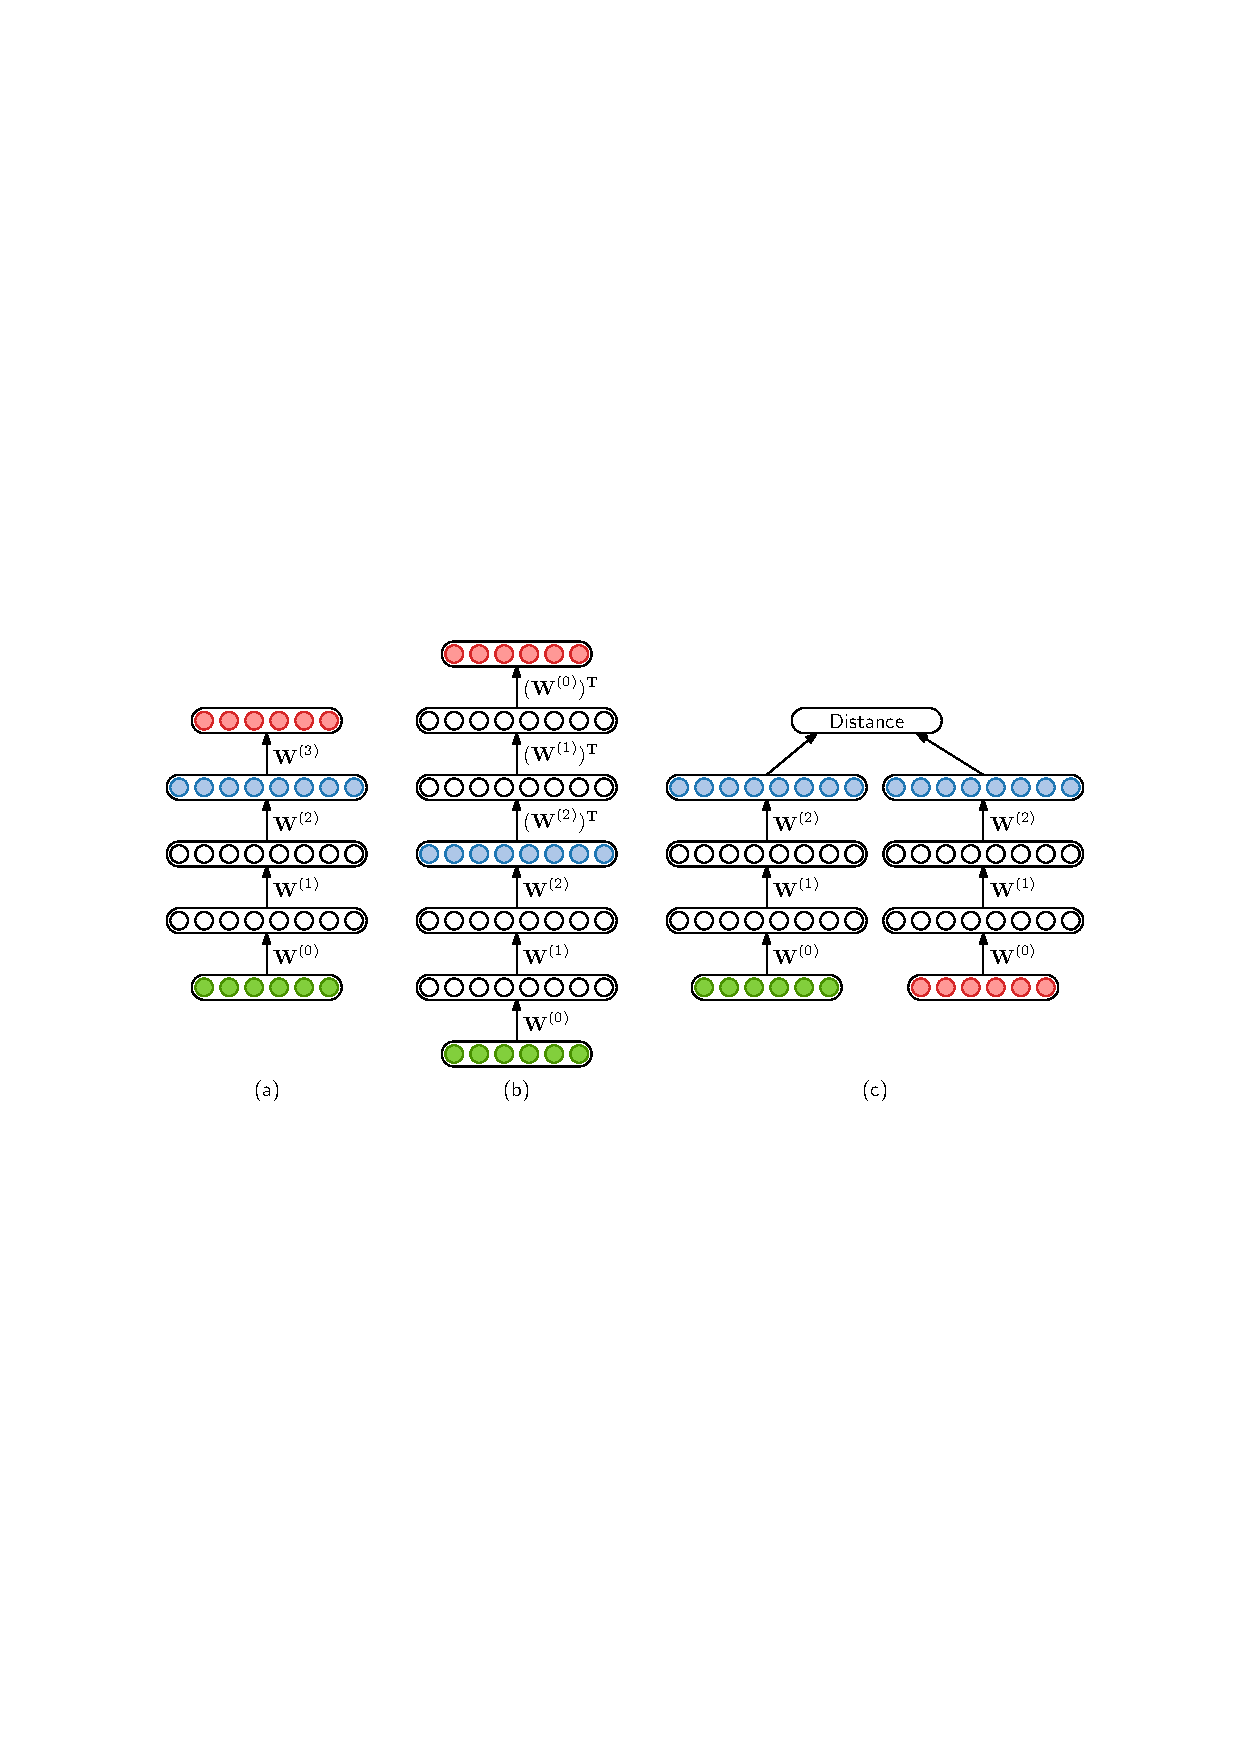
\includegraphics[width=\linewidth]{cae_siamese}
    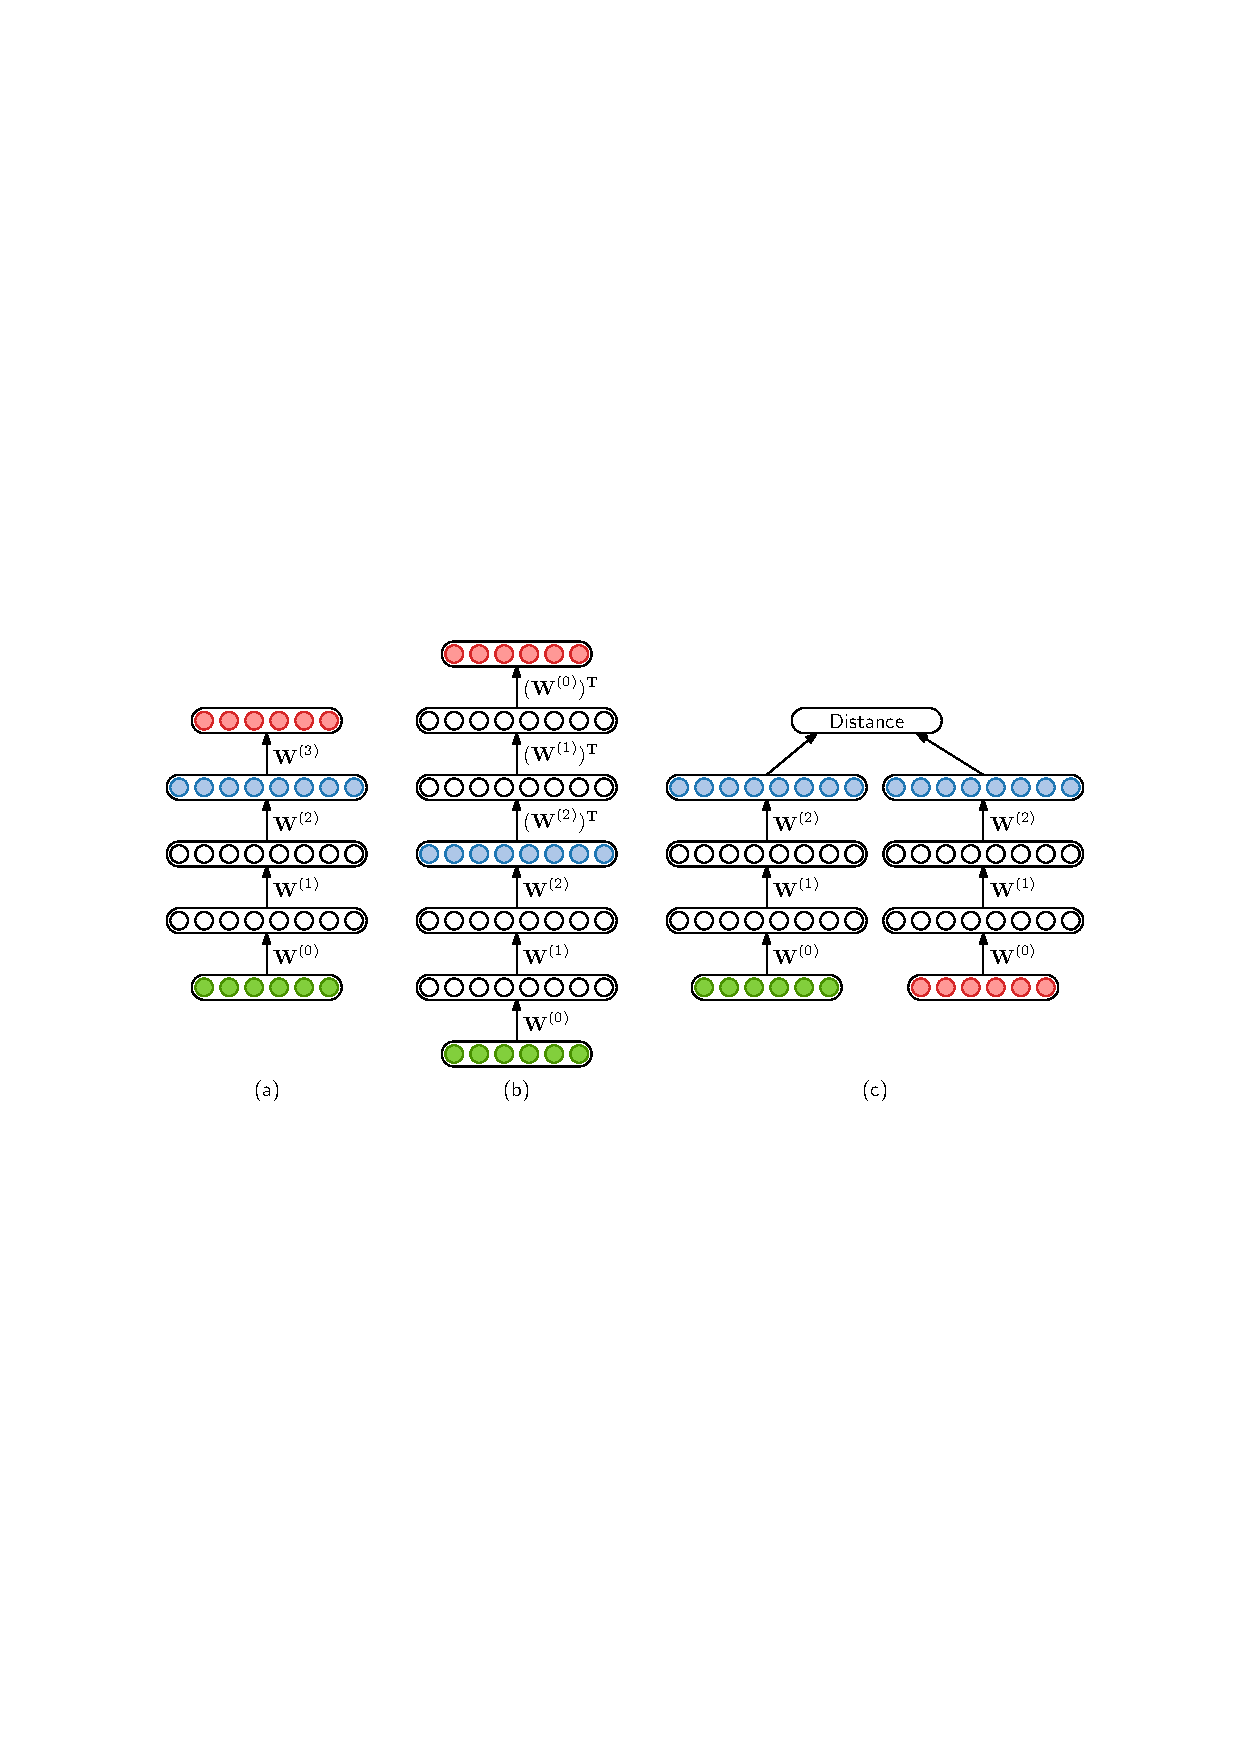
\includegraphics[width=0.918\linewidth]{cae_siamese}
    \caption[I am the short caption that appears in the list of figures, without references.]{
    (a) The cAE as used in this chapter. The encoding layer (blue) is chosen based on performance on a development set.
    (b) The cAE with symmetrical tied weights. The encoding from the middle layer (blue) is always used.
    (c) The siamese DNN. The cosine distance between aligned frames (green and red) is either minimized or maximized depending on whether the frames belong to the same (discovered) word or not.
    A cAE can be seen as a type of DNN~\cite{dahl+etal_taslp12}.
    }
    \label{fig:cae_siamese}
\end{figure}


The following is an example of an equation:
\begin{equation}
P(\vec{z} | \vec{\alpha}) = \int_{\vec{\pi}} P(\vec{z} | \vec{\pi}) \, p(\vec{\pi} | \vec{\alpha}) \, \textrm{d} \vec{\pi}
= \int_{\vec{\pi}} \prod_{k = 1}^K \pi_k^{N_k} \frac{1}{B(\vec{\alpha})} \prod_{k = 1}^K \pi_k^{\alpha_k - 1} \, \textrm{d} \vec{\pi}
\label{eq:example_equation}
\end{equation}
which you can subsequently refer to as~\eqref{eq:example_equation} or Equation~\ref{eq:example_equation}.
But make sure to consistently use the one or the other (and not mix the two ways of referring to equations).

\graphicspath{{literature/fig/}}

\chapter{Literature Review}
\label{chap:literature}

\subsection*{Introduction}

An attempt at advancing drought monitoring depends on a substantial foundation of prior research. Scholars have investigated methods ranging from traditional single-index approaches to more sophisticated probabilistic models. Notably, South Korean research has successfully employed Dynamic Naïve Bayes Classifiers (DNBCs) to develop composite drought indicators, and Hidden Markov Models (HMMs) have been used elsewhere to model drought dynamics. In contrast, the majority of South African studies concentrate on single indices for regional analyses, paying little attention to composite indicators. This review synthesises key contributions from these research areas to provide necessary context before continuing.

\subsection*{Development of a Multiple-Drought Index for Comprehensive Drought Risk Assessment Using a Dynamic Naive Bayesian Classifier}

In this study the authors developed a Dynamic Naive Bayesian Classifier multiple-drought index (DNBC-MDI) to produce a probabilistic, multi-dimensional assessment of drought risk. Their stated objectives were to combine conventional drought indices (SPI, SDI, ESI and WSCI) using a DNBC, to apply the resulting DNBC-MDI to bivariate drought-frequency analysis for risk estimation, and to investigate future changes in drought risk under an RCP8.5 climate scenario. Methodologically, the study focused on the Han River basin and used observed data for 1974–2016 together with synthetic climate projections for 2017–2099 generated by the HadGEM2-AO model under RCP8.5 scenario. The DNBC parameters were estimated with an expectation–maximisation (EM) algorithm using the \texttt{depmixS4} package from R. Bivariate drought frequency was assessed using a Clayton copula, and a risk equation was employed to compute 100-year return-period risks. The principal results showed that the DNBC-MDI achieved the highest average classification accuracy compared with the individual indices, whilst successfully reproducing several known drought episodes (1994–1995, 2001, 2008–2009, 2012, 2014–2015). The authors were very candid about their limitations, which are as follows: 
\begin{enumerate}
    \item The assessment focused predominantly on climate model outputs, disregarding remote-sensing products. For this they suggest using MODIS or Landsat.
    \item The model assumes conditional independence among the input indices. This assumption is brittle given the interconnections between precipitation, streamflow and evapotranspiration processes. 
\end{enumerate}
Overall, the paper demonstrates the technical feasibility and potential advantages of a DNBC-based composite indicator for drought characterisation. Simultaneously, it also signals important areas of concern with regards to robustness and transferability for an adaptation~\cite{dnbc_drought_second}.

\subsection*{Assessment of Probabilistic Multi-Index Drought Using a Dynamic Naive Bayesian Classifier}

This paper wanted to apply a DNBC to integrate multiple drought indices into a single, coherent drought state representation. The objectives were to combine indicators from different feature spaces, that being: SPI for meteorological, SDI for hydrological, and NVSWI for agricultural. Additionally, they wanted to evaluate whether the DNBC-based drought states could outperform individual indices in terms of detection, classification, and persistence. The study was carried out in the Han River upstream sub-basin in South Korea, using data from 1980–2015 for in-situ observations and 2003–2015 for MODIS-derived indices. The DNBC was constructed with five hidden drought states, the number selected using AIC, BIC and minimum log-likelihood for model selection criteria, and parameters were estimated through the EM algorithm implemented in the \texttt{depmixS4} R package.

The key results showed that the DNBC-based drought states successfully reproduced known drought episodes (2004, 2006, 2008–2009, 2014, 2015) and provided accurate representations of drought duration and persistence. In detection performance, DNBC-DS captured 100\%, 96\%, 100\%, and 93\% of droughts identified by SPI, SDI, NVSWI, and a composite drought index (CDI) respectively. The approach also highlighted the differing relationships between indicators, with strong correlation between SPI and SDI with a score of 0.648, but weak correlations involving NVSWI (0.186–0.187). Overall, the DNBC offered a probabilistic framework for drought monitoring that explicitly incorporated uncertainty, outperforming deterministic single-index approaches. 

Regardless, the authors acknowledged some of their key limitations. Firstly, the model relied on only three indices, which is not complex enough to capture what we call drought. It excluded potentially informative variables such as temperature, water vapour, and radiation. Beyond these, aligning with the paper above, this model also assumes that the input indices are conditionally independent once again making a brittle assumption.

Despite these constraints, the study offered a structured path toward a more holistic multi-indicator integration and contributed to the validity of using DNBCs for composite drought indicators~\cite{dnbc_drought_first}. 

\subsection*{Review of In-Situ and Remote Sensing-Based Indices and Their Applicability for Integrated Drought Monitoring in South Africa}

This study aimed to critically assess the performance and applicability of both in-situ and remote sensing-based drought indices for integrated drought monitoring in South Africa. Its objectives were to evaluate eight widely used indices and to determine which are most suitable for South Africa’s highly variable climate. These eight indices were: PDSI, SWSI, VCI, SPI, SPEI, SSI, SGI, and GRACE-based indices. A further aim was to test the hypothesis that no single index can adequately capture all aspects of meteorological, agricultural, and hydrological drought. 

They followed the World Meteorological Organisation’s (WMO) 2016 guidelines for drought indicator assessment. They used five evaluation criteria focusing on capability, sensitivity, data requirements, computational simplicity, and versatility for integration. The review drew from published studies in South Africa and other regions with similar climate characteristics. The indices were chosen based on surveys, while their feasibility was assessed against the evaluation framework mentioned. 

The findings demonstrated that the PDSI and SWSI are not feasible to obtain in South Africa due to their high complexity with regards to data requirements. However, SPI, SPEI, VCI, SSI, and SGI were identified as the most feasible candidates for integrated drought monitoring because of their simplicity and adaptability. Regardless, calculation issues remain, for example, there is no consensus on the most suitable probability distribution functions (PDF) for the calculations of SSI and SGI, with the most commonly used Gamma distribution performing poorly in South African catchments. Some alternative distributions showed improved results but inconsistencies persisted. Finally, the review recommended exploring multivariate approaches that combine SPI, SPEI, VCI, SSI, and SGI, while also noting the potential of GRACE-based indices, particularly with regards to groundwater, in order to compensate for the country’s limited groundwater records. 

The study transparently noted some important limitations. Data availability constraints undermine the feasibility of effective indices such as the PDSI and SGI, while the scarcity, or absence, of groundwater records limits applications. PDF selection for SSI and SGI remains uncertain given the climate variation in South Africa. The authors identified key research gaps within the nation, including the need for multivariate index testing and more exploration of GRACE-based products.

Ultimately, the review emphasised that integrated approaches, underpinned by sensitivity analysis and comparative testing, are required to strengthen drought monitoring in South Africa’s complex climatic landscape~\cite{za_drought_review}.

\subsection*{Developing a Composite Drought Indicator Using PCA Integration of CHIRPS Rainfall, Temperature, and Vegetation Health Products for Agricultural Drought Monitoring in New Mexico}

The objective of this study was to construct a Composite Drought Indicator for New Mexico, the so called CDI-NM, by integrating multiple variables through Principal Component Analysis (PCA). The research sought to provide a drought monitoring tool capable of identifying historical drought events, while also quantifying drought extent across the state. The study combined satellite-derived rainfall, temperature, and vegetation health products to demonstrate the effectiveness of PCA and to investigate drought impacts on agricultural production. 

The methodology focused on New Mexico which is an agriculturally important US state and is vulnerable to varying climates. Four input datasets spanning 2003–2019 were incorporated: CHIRPS rainfall data, MODIS Land Surface Temperature (LST), Smoothed Normalized Difference Vegetation Index (SMN), and Vegetation Condition Index (VCI). PCA was conducted independently for each month, with suitability being validated using Kaiser-Meyer-Olkin and Bartlett’s tests. They tested their model output by comparing it against SPI-3 and by correlating it with the annual variations in the yields of wheat, corn, peanuts, and cotton.

The results indicated that CDI-NM showed strong agreement with SPI-3, effectively capturing major drought events in 2003, 2011–2013, and 2018. Additionally, the showed their CDI-NM had strongly negative correlations with yields for corn (-0.68) and wheat (-0.63), while having a weaker correlation with cotton (-0.20). This reflects greater drought tolerance for cotton. Relationships between input variables were also consistent with expectation, as positive correlation was seen between VCI and rainfall (0.78) and negative correlation with LST (-0.43). Finally, the indicator demonstrated more natural variations than SPI, suggesting improved ability at capturing agricultural drought. 

Despite these achievements, several limitations were identified. The method of PCA relies on linear assumptions, temporal stationarity, and is sensitivity to scaling. The 17-year dataset is inherently limited with regards to long-term generalisability. Some data-related uncertainties further constrained precision. Redundancy between NDVI-derived SMN and VCI also posed risks of over-representation of vegetation conditions. Moreover, the study did not conduct sensitivity testing of PCA-derived weights, leaving gaps in applicability. The authors highlighted the need for longer datasets, uncertainty assessments, and more advanced dimensionality reduction techniques to strengthen the reliability of composite indicators for drought monitoring~\cite{atmos16070818}.

\subsection*{Conclusion}
The literature shows that probabilistic approaches are promising for capturing drought's complex nature, offering an advantage over traditional indices. Although South Korean research offers a strong blueprint, the scarcity of composite indicator development in South Africa reveals a significant research gap. This project seeks to bridge this gap by tailoring a DNBC to South Africa. 

\graphicspath{{methods/fig/}}

% TODO: DO THIS: Add implementation here as well like discretisation or whatever the fuck
\chapter{Methods}
\label{chap:methods}
\section{Data Acquisition}
The development of a composite drought indicator requires careful selection of input variables that capture the different aspects of drought. Three indices were selected: the Standardised Precipitation Index (SPI) to represent meteorological drought, the Streamflow Drought Index (SDI) to represent hydrological drought, and the Normalised Difference Vegetation Index (NDVI) as a proxy for agricultural drought. These indices were chosen based on their widespread use in literature and the availability of data. Data scarcity is a challenge in South Africa, as openly accessible, long and consistent drought-related datasets are limited. Consequently, the choice of indices attempts to strike a balance between theory and pragmatic constraints~\ref{za_drought_review,za_drought_review2,dnbc_drought_first,dnbc_drought_second}.

\ref{za_drought_review}


\subsection{Sources}
To compute the SPI, monthly rainfall data was obtained from the University of Cape Town (UCT) dataset, which covers the period 1979–2019 (Dataset~\ref{uct_data}). The dataset provides rainfall values at the station level, offering a high degree of spatial granularity across South Africa.

For the SDI, daily streamflow records were obtained from the Department of Water and Sanitation (DWS), which maintains audited historic data regarding hydrology (Dataset~\ref{DWS_2011}). These daily records were averaged to monthly to calculate the target index.

To obtain the NDVI, the NOAA Climate Data Record (CDR) of AVHRR Normalised Difference Vegetation Index (NDVI), Version~5 was used (Dataset~\ref{ndvi_data}). The dataset spans the period 1981–2025 and is provided in global NetCDF format. For the purposes of this study, only the South African subset was extracted. This required targeted downloading and filtering, given the large size of the global dataset.

\subsection{Preprocessing}


To prepare the indices for model input, several preprocessing steps were performed:  
\begin{enumerate}
    \item \textbf{Time Period Alignment:} All datasets were resampled or aggregated to a common monthly resolution.  
    \item \textbf{Area Alignment:} For station-based datasets, like rainfall and streamflow, records were harmonised by selecting stations with consistent temporal coverage. For NDVI, gridded data was averaged over the area of choice. 
    \item \textbf{Brief Exploration Of Data:} The data sets were analysed to identify and issues in the data such as missing/null values, format consistency, validity, etc. No problems were found
\end{enumerate}

\section{Index Calculation}
\label{sec:index-calc}

The selected datasets were subsequently transformed into drought indices using established methodologies. The SPI was derived from rainfall anomalies through standardisation against a long-term climatology. The SDI was computed by standardising streamflow anomalies relative to long-term hydrological records. The NDVI, while not a drought index in its raw form, was used to reflect vegetation stress associated with agricultural drought conditions. References to the seminal works underlying these methodologies are provided in the bibliography.

\subsection{SPI}

The SPI is based on the statistical normalisation of accumulated precipitation over a specified time window. Precipitation values are first fitted to a probability distribution, commonly the gamma distribution, and then transformed into a standard normal distribution. This yields an index with mean zero and unit variance, allowing for direct interpretation of drought severity across different temporal scales.

\subsection{SDI}

The SDI extends the concept of the SPI to streamflow. It is calculated by aggregating streamflow over a specified time window and standardising it against long-term flow records. Positive values of SDI indicate above-normal hydrological conditions, while negative values reflect hydrological drought. The SDI is particularly relevant in South Africa, where surface water storage and river systems play a critical role in drought impact and management.

\subsection{NDVI}

The NDVI is derived from remotely sensed reflectance in the red and near-infrared bands of the electromagnetic spectrum. Vegetated surfaces typically absorb red light for photosynthesis and reflect near-infrared light, making the NDVI an effective indicator of vegetation health. While NDVI is not a drought index per se, reductions in NDVI are widely used to monitor agricultural drought stress, as vegetation is sensitive to deficits in soil moisture and precipitation.

\subsection{Discretisation of Indices}

The SPI, SDI, and NDVI are all continuous variables. However, the Dynamic Naïve Bayes Classifier requires discrete inputs. Accordingly, each index was discretised into categorical bins based on thresholds reported in the literature and common practice. For example, SPI values are often classified into categories such as “extremely dry,” “moderately dry,” and “normal.” This discretisation not only facilitates model implementation but also aligns with the interpretive categories commonly employed in drought monitoring. A more detailed account of the discretisation procedure is provided in Section~\ref{sec:implementation}.

\begin{table}[h]
\centering
\caption{Discretisation thresholds for drought indices.}
\label{tab:discretisation}
\begin{tabular}{lccc}
\toprule
\textbf{Category} & \textbf{SPI / SDI} & \textbf{NDVI Anomaly} & \textbf{Interpretation} \\
\midrule
Severe Drought    & $\leq -1.5$        & $\leq -1.5$          & Extreme vegetation/hydrological stress \\
Moderate Drought  & $-1.5 < x \leq -0.5$ & $-1.5 < x \leq -0.5$ & Sustained but moderate deficit \\
Normal            & $-0.5 < x < 0.5$  & $-0.5 < x < 0.5$     & Near-average conditions \\
Moderate Wet      & $0.5 \leq x < 1.5$ & $0.5 \leq x < 1.5$   & Above-average moisture/greenness \\
Severe Wet        & $\geq 1.5$        & $\geq 1.5$           & Flooding risk or excessive rainfall \\
\bottomrule
\end{tabular}
\end{table}

\section{Model Development}
\subsection{Model Design}

\subsubsection{Defining the Random Variables}

The proposed DNBC is constructed in a general form with $N$ input variables observed across $T$ discrete time steps. All random variables (RVs) in the model are treated as discrete.  

The first set of RVs corresponds to the latent drought states at each time step, denoted by
\[
S_t \in \{1,2,\dots,m\}, \quad t = 1, \dots, T,
\]
where $m$ represents the number of possible drought states. This value of $m$ is not fixed, but will rather be determined via model selection.  

The second set of RVs corresponds to the observed input variables, denoted by
\[
A_t^{(n)} \in \{1,2,\dots,C_n\}, \quad n = 1, \dots, N, \quad t = 1, \dots, T,
\]
where $C_n$ is the cardinality of the $n$-th input variable. In this project, these inputs are the indices used to represent different aspects of drought:
\[
\text{SPI} \equiv A_t^{(1)}, \quad 
\text{SDI} \equiv A_t^{(2)}, \quad 
\text{NDVI} \equiv A_t^{(3)}.
\]
These observed indices constitute the data set $\mathcal{D}$.  

For clarity, we define the following notation which will be used throughout the model formulation:
\[
\vec{S}_{1:T} = \{S_1, S_2, \dots, S_T\}, \quad 
A_{1:T} = \{\vec{A}_1, \vec{A}_2, \dots, \vec{A}_T\},
\]
where each $\vec{A}_t = \{A_t^{(1)}, A_t^{(2)}, \dots, A_t^{(N)}\}$.  

The total number of latent state nodes is therefore $T$, while the number of observed input nodes is $T \times N$. A summary of the random variables, their number of nodes, and their cardinality is provided in Table~\ref{tab:RVs}.

\begin{table}[H]
\centering
\caption{Summary of random variables in the model}
\label{tab:RVs}
\begin{tabular}{lcc}
\hline
\textbf{Name} & \textbf{Number of Nodes} & \textbf{Cardinality} \\ \hline
Latent drought state $S_t$ & $T$ & $m$ \\
General input variable $A_t^{(n)}$ & $T \times N$ & $C_n$ \\
\hline
\end{tabular}
\end{table}

\subsubsection{Graphical Structure \& Assumptions}

Figure~\ref{fig:dnbc-diagram} below displays the model diagram for a DNBC for $T$ time steps and $N$ input variables.  

\begin{figure}[!h]
    \centering
    \includegraphics[width=\linewidth]{dnbc-diagram.png}
    \caption[TODO]{
The Dynamic Naïve Bayes Classifier (DNBC) can be represented as a Bayesian network unfolding over time. At each time step $t$, a latent drought state $S_t$ is modelled as a discrete random variable that governs the latent structure, while the observed input variables $\vec{A}_t = \{A_t^{(1)}, A_t^{(2)}, \dots, A_t^{(N)}\}$ are each solely dependent on $S_t$}
    \label{fig:dnbc-diagram}
\end{figure}

It is important to note the inherent limitations of this model, that being:
\begin{enumerate}[label=(\roman*)]
    \item The dynamic process of the state sequence $S_t$ follows a first-order Markov chain. This means the state at time $t+1$ is conditionally dependent only on the state at time $t$. \label{item:assumption_1}
    \item The dynamic process is stationary, implying that the transition probabilities between states are constant over time. \label{item:assumption_2}
    \item For each time step $t$, the model assumes conditional independence among the input variables $\vec{A}_t$ given the corresponding hidden drought state $S_t$. \label{item:assumption_3}
\end{enumerate}

\subsubsection{Joint Distribution}

The joint probability distribution of the observed variables and latent states in the DNBC can be expressed as:
\begin{equation}
    \begin{align}
        p(S_1, &S_2, \dots, S_T, A^{(1)}_1, A^{(2)}_1, \dots, A^{(N)}_1, A^{(1)}_2, \dots, A^{(N)}_T) \\ 
        &= p(S_1, S_2, \dots, S_T, \vec{A}_1, \vec{A}_2, \dots, \vec{A}_T) \\
        &= p(\vec{S}_{1:T}, A_{1:T}) \\
        &= p(S_1) \cdot \prod\limits_{t=1}^{T-1} p(S_{t+1} \mid S_t) \cdot \prod\limits_{n=1}^{N} \prod\limits_{t=1}^T p(A^{(n)}_t \mid S_t)
    \end{align}
    \label{eqn:joint_distr}
\end{equation}

The following factorisation is possible due to Assumption~\ref{item:assumption_3} of the DNBC and will become useful at a later stage.
\begin{equation} 
    \begin{align} 
        p(\vec{A}_{t} \mid S_t) &= p(A_t^{(1)}, A_t^{(2)}, \dots, A_t^{(N)} \mid S_t) \\ 
        &= p(A_t^{(1)} \mid S_t)p(A_t^{(2)} \mid S_t)\dotsp(A_t^{(N)} \mid S_t) \\ 
        &= \prod\limits_{n=1}^N p(A_t^{(n)} \mid S_t) 
    \end{align} 
    \label{eqn:attribute_rv_factorisation} 
\end{equation}

\subsubsection{Parameterising the Model}
The DNBC is fully specified by three sets of parameters, that being the prior, transition and emission probabilities. 

\paragraph{Prior Probabilities:}  
The initial distribution over the latent drought $S_1$. \\
The factor table for the priors is show below in Table~\ref{tbl:priors_factor_table}:
\begin{table}[!h]
    \mytable
    \caption{Priors Factor Table}
    \begin{array}{c | c}
        S_1 & p(S_1) \\ 
        \hline
        1 & \pi_1 \\ 
        2 & \pi_2 \\ 
        \vdots & \vdots \\
        m & \pi_m \\ 
    \end{array} 
    \label{tbl:priors_factor_table}
\end{table}

where $\pi_i$ is the probability that the system begins in state $i$. 
\[
\pi_i \equiv p(S_1 = i),
\]

\paragraph{Transition Probabilities:}  
defines the likelihood of moving to a new hidden state given the current hidden state. \\
The factor table as well as the transition matrix $P^1$ is shows below in Table~\ref{tbl:transition_factor_table}:

\begin{table}[!h]
    \mytable
    \caption{Transition Factor Table \& Transition Matrix}
        \begin{array}{ccc}
        \begin{array}{c c | c}
        S_t & S_{t+1} & p(S_{t+1} \mid S_t) \\ 
        \hline
        1 & 1  & a_{1,1} \\ 
        1 & 2  & a_{1,2} \\ 
        \vdots & \vdots  & \vdots \\
        1 & m  & a_{1, m} \\ 
        2 & 1  & a_{2, 1} \\ 
        2 & 2  & a_{2, 2} \\ 
        \vdots & \vdots  & \vdots \\
        m & m  & a_{m,m} \\ 
        \end{array} 
        &
        \equiv
        &
        P^1 = 
        \begin{bmatrix}
        a_{1,1} & a_{1,2} & \dots & a_{1,m} \\
        a_{2,1} & a_{2,2} & \dots & a_{2,m} \\
        \vdots & \vdots & \ddots & \vdots \\
        a_{m,1} & a_{m,2} & \dots & a_{m,m} \\
        \end{bmatrix}
        \end{array} 
    \label{tbl:transition_factor_table}
\end{table}

Here, $a_{i,j}$ represents the probability of transitioning from state $i$ at time $t$ to state $j$ at time $t+1$. 
\[
a_{i,j} \equiv p(S_{t+1} = j \mid S_t = i).
\]
Note as well that transition matrix's rows sum to $1$, ie. $\sum_{j=1}^m a_{i,j} = 1$ for all $i$.  

\paragraph{Emission Probabilities:}  
Defines the likelihood of observing a particular inout variable, given that the system is in a specific hidden state. \\
Once again, the factor table for the emission probabilities is show below in Table~\ref{tbl:emission_factor_table}
\begin{table}[!h]
    \mytable
    \caption{Emission Factor Table}
        \begin{array}{c c | c}
        A^{(n)}_t & S_t & p(A^{(n)}_t \mid S_t) \\ 
        \hline
        1 & 1  & b_1^{(n)}(1) \\ 
        1 & 2  & b_2^{(n)}(1) \\ 
        \vdots & \vdots  & \vdots \\
        1 & m  & b_m^{(n)}(1) \\ 
        2 & 1  & b_1^{(n)}(2) \\ 
        2 & 2  & b_2^{(n)}(2) \\ 
        \vdots & \vdots  & \vdots \\
        C_n & m  & b_m^{(n)}(C_n) \\ 
        \end{array} 
    \label{tbl:emission_factor_table}
\end{table}

Where, $b_i^{(n)}(j)$ is the likelihood of observing input variable $n$ take on the value $j$, given the its corresponding hidden drought state is equal to $i$
\[
b_i^{(n)}(j) \equiv p(A_t^{(n)} = j \mid S_t = i).
\]

These parameters encode how the drought indicators behave under each latent drought state.  
Taken together, the parameter set fully determines the DNBC. It is important to note that due to the parameters being time independent, as the model assumes stationarity, the rules governing drought state transitions and emissions are invariant across time.

\subsection{Inference}
\label{sec:inference}

In this section, inference for the DNBC is developed under the assumption that the parameters $\Theta$ are known and the input variables $A_{1:T}$ are observed. Since the attributes are not random at this stage, the task becomes trying to infer the distribution of the hidden drought states:
\[
    p(\vec{S}_{1:T} \mid A_{1:T}, \Theta),
\]
This will later be used for the E-step in the EM algorithm.

The inference procedure is carried out using the Junction Tree (JT) framework, which provides exact inference. Messages are propagated through the tree, beginning at the leaf clusters and moving inward~\cite{lauritzen1988local}. \\
Figure~\ref{fig:jt_diagram} illustrates the JT structure associated with the DNBC.

\begin{figure}[!h]
    \centering
    \includegraphics[width=\linewidth]{jt-diagram.png}
    \caption{Junction Tree representation of the DNBC. Each cluster groups together latent state variables and observed attributes, with sepsets defined along the edges. Messages are propagated through the tree to perform exact inference.}
    \label{fig:jt_diagram}
\end{figure}
It is useful to note the factorisation of the observed attribute RVs at Equation~\ref{eqn:attribute_rv_factorisation}.

The cluster potentials are summarised in Table~\ref{tbl:cluster_potentials}.
\begin{table}[!h]
    \mytable
    \caption{Cluster potentials for the DNBC. Each potential corresponds either to a state transition or to a state-attribute relationship.}
    \begin{aligned}[c]
        &- \\
        \psi_2(S_1, S_2) &= p(S_2 \mid S_1) \\
        &\vdots \\
        \psi_t(S_{t-1}, S_t) &= p(S_t \mid S_{t-1}) \\
        &\vdots \\
        \psi_T(S_{T-1}, S_T) &= p(S_T \mid S_{T-1}) \\
    \end{aligned}
    \qquad \qquad \qquad
    \begin{aligned}[c]
        \psi_1(S_1, \vec{A}_1) &= p(S_1)p(\vec{A}_1 \mid S_1) \\
        \psi_2(S_2, \vec{A}_2) &= p(\vec{A}_2 \mid S_2) \\
        &\vdots \\
        \psi_t(S_t, \vec{A}_t) &= p(\vec{A}_t \mid S_t) \\
        &\vdots \\
        \psi_T(S_T, \vec{A}_T) &= p(\vec{A}_T \mid S_T) \\
    \end{aligned}
    \label{tbl:cluster_potentials}
\end{table}

\subsubsection{Message Passing}
Messages are defined between clusters, with sepsets given by the product of messages between clusters. 

\paragraph{Upward messages:}  
Because the attributes are observed, upward messages collapse to the corresponding likelihood terms.
\begin{align*}
    \delta_{t\uparrow} (S_t) &= \sum\limits_{\vec{A}_t} \psi_t(S_t, \vec{A}_t) \\ 
    &= \sum\limits_{\vec{A}_t} p(\vec{A}_t \mid S_t) \\
    &= p(\vec{A}_t \mid S_t)
\end{align*}
since marginalisation over the observed attributes reduces to their likelihood.


\paragraph{Rightward messages:}  
Rightward propagation starts at the leftmost cluster and moves forward in time:
\begin{align*} 
    \delta_{1 \rightarrow 2} (S_1) &= \sum\limits_{\vec{A}_1} \psi_1(S_1, \vec{A}_1) \\
    &= \sum\limits_{\vec{A}_1} p(S_1)p(\vec{A}_1 \mid S_1) \\
    &= p(S_1)p(\vec{A}_1 \mid S_1) \numberthis \label{eqn:rightward_message_init} \\
    \\
    \delta_{t \rightarrow t+1} (S_t) &= \sum\limits_{S_{t-1}} \psi_t(S_{t-1}, S_t) \delta_{t-1 \rightarrow t}(S_{t-1}) \delta_{t\uparrow}(S_t) \\
    &= \sum\limits_{S_{t-1}} p(S_t \mid S_{t-1}) \delta_{{t-1} \rightarrow t}(S_{t-1}) p(\vec{A}_t \mid S_t) \\
    &= p(\vec{A}_t \mid S_t) \sum\limits_{S_{t-1}} p(S_t \mid S_{t-1}) \delta_{{t-1} \rightarrow t}(S_{t-1}) \numberthis \label{eqn:rightward_message_final} \\
\end{align*}

\paragraph{Leftward messages.}  
Similarly, leftward propagation begins at the final cluster and proceeds backward:
\begin{align*} 
    \delta_{T-1 \leftarrow T} (S_{T-1}) &= \sum\limits_{S_T} p(S_T \mid S_{T-1})p(\vec{A}_T \mid S_T), \numberthis \label{eqn:leftward_message_init} \\
    \\
    \delta_{t-1 \leftarrow t} (S_{t-1}) &= \sum\limits_{S_t} p(S_t \mid S_{t-1}) \delta_{t \leftarrow t+1}(S_t) p(\vec{A}_t \mid S_t). \numberthis \label{eqn:leftward_message_final}
\end{align*}

\subsubsection{Remarks}
In this framework, the clusters of primary interest are $\psi_t(S_t, S_{t+1})$ and the sepsets $\mu_{t,t+1}(S_t)$, which directly contribute to the computation of $p(\vec{S}_{1:T} \mid A_{1:T}, \Theta)$. As a result, downward messages (e.g., from $\psi_t(S_{t-1}, S_t)$ to $\psi_t(S_t, \vec{A}_t)$) are not of interest. \\
Finally, it is worth noting that for JTs, since the underlying graph is a tree, message passing is exact. We follow a specific message-passing ordering of the standard Belief Propagation algorithm, which is guaranteed to converge to the exact marginals.

\subsubsection{Forward–Backward Algorithm}
At this point, it is natural to highlight the connection between the JT approach described above and the more classical algorithms for HMMs along with their variants. Readers familiar with the literature will recognise that the message passing operations we performed are precisely the equivalent to the well-known \emph{forward–backward equations}~\cite{binder1997space,wiki:forward_backward,aviles}. \\
The forward and backward recursions applied to the proposed model are shown below:

\paragraph{Forward:}
\begin{flalign}
    &\qquad \text{Define:} \qquad \alpha_t^k = p(A_{1:t}, S_t = i)& \nonumber \\
    &\qquad \text{Init:} \qquad \alpha_1^k = p(S_1 = k)p(\vec{A}_1 \mid S_1 = k)& \nonumber \\
    &\qquad \text{Iteration:} \qquad \alpha_t^k = p(\vec{A}_t \mid S_t = k)\sum\limits_{i=1}^m \alpha_{t-1}^i \cdot p(S_t = k \mid S_{t-1} = i)& \label{eqn:forward_eqn}
\end{flalign}

\paragraph{Backward:}
\begin{flalign}
    &\qquad \text{Define:} \qquad \beta^k_t = p(A_{1:t}, S_t = i)& \nonumber \\
    &\qquad \text{Init:} \qquad \beta^k_T = 1 \quad \forall \, k& \nonumber \\
    &\qquad \text{Iteration:} \qquad \beta^k_t = \sum\limits_{i=1}^m p(S_{t+1} = i \mid S_t = k) \cdot p(\vec{A}_{t+1} \mid S_{t+1} = i) \cdot \beta_{t+1}^i& \label{eqn:backward_eqn}
\end{flalign}

\subsubsection*{Remarks on Forward–Backward and Baum–Welch}
The messages passed in the JT (Equations~\ref{eqn:rightward_message_init} - \ref{eqn:leftward_message_final}) coincide with the $\alpha$ and $\beta$ recursions in Equations~\ref{eqn:forward_eqn}–\ref{eqn:backward_eqn}. The distinction is thus in presentation alone. The JT framework is a generalisation for arbitrary graphical models, whereas the forward–backward is the special case formulation for the structure of HMMs\cite{hmm_slides}.

It is worth emphasising the parallel between the JT messages and the forward–backward quantities. The forward recursion $\alpha_t^k=p(A_{1:t},S_t=k)$ and the backward recursion $\mathit{\beta_t^k=p(A_{t+1:T}\mid S_t=k)}$ are algebraically equivalent to the inward and outward sum–product messages in the JT~\ref{fig:jt_diagram}. When inward and outward messages are combined at a cluster or sepset, the resulting posterior marginals $p(S_t \mid A_{1:T})$ and pairwise marginals $p(S_t,S_{t+1}\mid A_{1:T})$ coincide with the responsibilities computed from Baum-Welch. Thus, the JT message-passing procedure and the forward–backward algorithm produce identical posterior marginals. These results will be of interest in the following sub section for parameter estimation~\cite{aviles,dnbc_drought_first,hmm_slides,wiki:baum_welch}.

In summary, the JT formulation highlights the structural perspective, while forward–backward and Baum–Welch remain the traditional algorithms in the literature. Both views are mathematically equivalent and lead to the same computations.

\subsection{Parameter Estimation}
Parameter estimation for the DNBC is carried out using the Expectation–Maximization (EM) algorithm~\cite{moon_tk}.  
We distinguish between the hidden variables, observed data, and model parameters as follows:

\begin{align*}
    \mathcal{H} &= (S_t)_{t=1}^T  \\
    \mathcal{D} &= (\vec{A}_t)_{t=1}^T  \\
    \Theta &= (\vec{\theta}_1, \vec{\theta}_2, \vec{\theta}_3)  \\
    \text{Whe}& \text{re,} \\
     & \quad \vec{\theta}_1 = \{\pi_1, \pi_2, \dots, \pi_m\} \equiv \text{Priors Probabilities}  \\
     & \quad \vec{\theta}_2 = \{a_{i,j} \mid i,j = 1, \dots, m\} \equiv \text{Transition Probabilities}  \\
     & \quad \vec{\theta}_3 = \left\{ b_i^{(n)}(j) \,\middle|\, i = 1,\dots,m; \, n = 1,\dots,N; \, j = 1,\dots,C_n \right\} \equiv \text{Emission Probabilities} 
\end{align*}

The EM algorithm iteratively alternates between two steps:

\subsubsection{1. E-Step}

In this step, we hold $\Theta$ fixed and compute the posterior distribution over the hidden states:

\begin{align}
    q(\mathcal{H}) &= p(\mathcal{H} \mid \mathcal{D}, \Theta) \nonumber \\
    &= p(\vec{S}_{1:T} \mid A_{1:T}, \Theta) \numberthis \label{eqn:e_step}
\end{align}

This corresponds directly to the inference problem, as previously discussed in Section~\ref{sec:inference}.

\subsubsection{2. M-Step}

Next, with $q$ fixed, we maximise the variational lower bound
\[
    \mathscr{L}(q, \Theta) = \sum\limits_{\mathcal{H}}q(\mathcal{H}) \cdot \log \left( \frac{p(\mathcal{D}, \; \mathcal{H} \mid \Theta)}{q(\mathcal{H})} \right)
\]
with respect to $\Theta$.

Equivalently, this requires solving
\begin{align}
    \Theta &= \underset{\Theta}{\operatorname{argmax}} \; \mathcal{Q}(\Theta) \nonumber \\
    &= \underset{\Theta}{\operatorname{argmax}} \sum\limits_{\mathcal{H}} q(\mathcal{H}) \cdot \log \, p(\mathcal{D}, \mathcal{H} \mid \Theta) \numberthis \label{eqn:m_step}
\end{align}

The inner term, $\log \, p(\mathcal{D}, \mathcal{H} \mid \Theta)$, is simply the log of the joint distribution introduced in Equation~\ref{eqn:joint_distr}. Expanding this expression yields:
\begin{align*}
    p(A_{1:T} \, \vec{S}_{1:T} \mid \Theta) &= \log \, p(S_1 \mid \vec{\theta}_1) \\ 
    &\qquad + \sum\limits_{t=1}^{T-1} \log \, p(S_{t+1} \mid S_t, \, \vec{\theta}_2) \\ 
    &\qquad + \sum\limits_{n=1}^N \sum\limits_{t=1}^T \log \, p(A_t^{(n)} \mid S_t, \, \vec{\theta}_3) 
\end{align*}

Substituting this into $\mathcal{Q}(\Theta)$ and carefully reorganising terms allows us to isolate contributions from priors, transitions, and emissions. Since all RVs are discrete, probabilities translate directly into parameterised forms, and the optimisation decouples naturally across $\vec{\theta}_1, \vec{\theta}_2$, and $\vec{\theta}_3$.

\begin{align*}
    \mathcal{Q} &= \sum\limits_{\mathcal{H}} q(\mathcal{H}) \cdot \log \, p(\mathcal{D}, \mathcal{H} \mid \Theta) \\
    &= \sum\limits_{\mathcal{H}} q(\mathcal{H}) \cdot \bigr[ \log \, p(S_1 \mid \vec{\theta}_1) \\ 
    &\qquad \qquad \qquad + \sum\limits_{t=1}^{T-1} \log \, p(S_{t+1} \mid S_t, \, \vec{\theta}_2) \\ 
    &\qquad \qquad \qquad + \sum\limits_{n=1}^N \sum\limits_{t=1}^T \log \, p(A_t^{(n)} \mid S_t, \, \vec{\theta}_3) \bigr]
\end{align*}

We then multiply $\sum\limits_{\mathcal{H}} q(\mathcal{H})$ through, understanding that $\mathcal{H} = (S_1, \dots, S_T)$
\begin{align*}
    &= \sum\limits_{S_1, \dots, S_T} \log \, p(S_1 \mid \vec{\theta}_1) \, q(S_1, \dots, S_T) \\ 
    & \qquad + \sum\limits_{S_1, \dots, S_T} \sum\limits_{t=1}^{T-1} \log \, p(S_{t+1} \mid S_t, \, \vec{\theta}_2) \, q(S_1, \dots, S_T) \\ 
    &\qquad + \sum\limits_{S_1, \dots, S_T} \sum\limits_{n=1}^N \sum\limits_{t=1}^T \log \, p(A_t^{(n)} \mid S_t, \, \vec{\theta}_3) \, q(S_1, \dots, S_T) \\
    \\
    &= \sum\limits_{S_1} \log \, p(S_1 \mid \vec{\theta}_1) \, q(S_1) + \sum\limits_{S_2, \dots, S_T} q(S_2, \dots, S_T) \\ 
    & \qquad + \sum\limits_{t=1}^{T-1} \sum\limits_{S_t, S_{t+1}} \log \, p(S_{t+1} \mid S_t, \, \vec{\theta}_2) \, q(S_t, S_{t+1}) + \sum_{\substack{S_1,\dots, S_T \\ \setminus S_t, \, S_{t+1}}} q(S_1, \dots, S_T) \\ 
    &\qquad + \sum\limits_{n=1}^N \sum\limits_{t=1}^T \sum\limits_{S_t} \log \, p(A_t^{(n)} \mid S_t, \, \vec{\theta}_3) \, q(S_t) + \sum_{\substack{S_1,\dots, S_T \\ \setminus S_t}} q(S_1, \dots, S_T) \\
\end{align*}

Since the goal is to optimise w.r.t $\Theta = (\vec{\theta}_1,\vec{\theta}_2,\vec{\theta}_3)$, all the terms not involving $\Theta$ can be dropped, whilst also using the result $\sum\limits_{S_t} p(S_t) = \sum\limits_{i=1}^m p(S_t = i)$
\begin{align*}
    &= \sum\limits_{i=1}^m \log \, p(S_1 = i \mid \vec{\theta}_1) \, q(S_1 = i) \\
    & \qquad + \sum\limits_{t=1}^{T-1} \sum\limits_{i=1}^m \sum\limits_{j=1}^m \log \, p(S_{t+1} = j \mid S_t = i, \, \vec{\theta}_2) \, q(S_t = i, S_{t+1} = j) \\
    &\qquad + \sum\limits_{n=1}^N \sum\limits_{t=1}^T \sum\limits_{i=1}^m \log \, p(A_t^{(n)} \mid S_t = i, \, \vec{\theta}_3) \, q(S_t = i) \\
\end{align*}

This representation can be expressed in terms of the model parameters. Because all random variables are discrete, the probabilities naturally reduce to combinations of these parameters.
\begin{align*}
    &= \sum_{i=1}^m q(S_1 = i) \log \pi_i \\
    &\qquad + \sum_{t=1}^{T-1}\sum_{i=1}^m\sum_{j=1}^m q(S_t=i,S_{t+1}=j)\log a_{i,j}\\ 
    &\qquad +  \sum\limits_{t=1}^T \sum\limits_{i=1}^m  q(S_t = i)  \sum\limits_{n=1}^N \log b_i^{(n)}(A_t^{(n)}) \\
\end{align*}

Each of the target parameters are now separated into their own terms and thus can be easily optimised in isolation. This yields the standard re-estimation updates~\cite{jm3,xing_slides}:
\begin{equation}
    \boxed{\;\pi_i^{\text{new}} = q(S_1=i)\;}
    \label{eqn:prior_update_rule}
\end{equation}
\begin{equation}
    \boxed{\;a_{i,j}^{\text{new}}=\frac{\sum\limits_{t=1}^{T-1} q(S_t=i,S_{t+1}=j)}{\sum\limits_{t=1}^{T-1} q(S_t=i)}\;}
    \label{eqn:transition_update_rule}
\end{equation}
\begin{equation}
    \boxed{\; b_i^{(n)}(j)^{\text{new}} = \frac{\sum\limits_{t=1}^T q(S_t = i) \cdot \mathbf{1}(A_t^{(n)} = j)}{\sum\limits_{t=1}^T q(S_t = i)} \;}
    \label{eqn:emission_update_rule}
\end{equation}

\subsection{Model Selection}
Model selection will involve determining the appropriate cardinality of each latent drought states $S_t$, that is, determining the value of $m$. When selecting $m$, a balance must be struck between model complexity and goodness of fit, as a larger value of $m$ gives the model a greater ability to capture subtle drought dynamics but risks overfitting. On the other hand, a smaller number may be too restrictive to reflect the underlying processes.

To guide this choice, three complementary criteria are applied: the Akaike Information Criterion (AIC), the Bayesian Information Criterion (BIC), and the maximised log-likelihood of the fitted model. These are given by
\begin{align}
    AIC &= -2 \cdot \log L(\Theta) + 2p, \label{eqn:aic}\\
    BIC &= -2 \cdot \log L(\Theta) + p \cdot \log k, \label{eqn:bic}
\end{align}
where $L(\Theta)$ is the maximised value of the likelihood function, $p$ is the number of free parameters in the model, and $k$ is the number of data points.  

The philosophy underlying these criteria is rooted in Occam’s razor, which is often phrased as ”the simplest
explanation is usually the best one”. AIC and BIC both balance model fit against complexity, but with differing severity. BIC applies a stronger penalty on complexity and is thus generally considered more consistent with Occam’s razor~\cite{Barber_2012}. Thus, the framework for selecting $m$ as follows:
\begin{enumerate}
    \item \textbf{Primary:} select the model with the lowest BIC, penalising unnecessary complexity.
    \item \textbf{Secondary:} use AIC to cross-check results.
    \item \textbf{Tertiary:} inspect the log-likelihood curve. If $\log L(\Theta)$ improves only marginally as $m$ increases, the simpler model is preferred (the so-called “elbow rule”).
\end{enumerate}

In practice, model selection is performed by sweeping across candidate values of $m$, fitting a model for each case, and comparing their AIC, BIC, and log-likelihood values. The final choice of $m$ seeks to minimise both AIC and BIC while ensuring that the likelihood $L(\Theta)$ does not deteriorate substantially.

\subsubsection{Choice of $k$}

The term $k$ in~\eqref{eqn:bic} represents the number of data points. Following common practice in the literature and implementation libraries such as the \texttt{seqHMM} package in R~\cite{cran_hmmSeq}, $k$ is calculated as: 
\[
    k = T \times N,
\]

\subsubsection{Number of Free Parameters $p$}

The number of free parameters $p$ corresponds to the model’s degrees of freedom. This includes contributions from the prior probabilities~\ref{tbl:priors_factor_table}, the transition probabilities~\ref{tbl:transition_factor_table}, and the emission probabilities~\ref{tbl:emission_factor_table}. It is widely accepted in the literature and implementations regarding HMMs and its variants~\cite{cran_hmmSeq,free_params_slides} that
\begin{align*}
    p &= (m-1) + m(m-1) + \sum_{n=1}^N m(C_n - 1) \\
      &= m^2 - 1 + m \sum_{n=1}^N (C_n - 1),
\end{align*}

\subsubsection{Log-Likelihood Estimation}

The third component of model selection is the log-likelihood, $\ell(\Theta)$, which measures the probability of the observed data under the model parameters:
\[
    \ell(\Theta) = p(A_{1:T}^\text{obs} \mid \Theta).
\]

This likelihood can be evaluated efficiently using the forward algorithm. Recall that the forward variable is defined as
\[
    \alpha_t^k = p(S_t = k, A_{1:t} \mid \Theta),
\]
The overall likelihood is then simply obtained by marginalising over the latent state at the final time step:
\begin{align*}
    \sum_{i=1}^m \alpha_T^i &= \sum_{S_T} p(A_{1:T}, S_T \mid \Theta) \\
                             &= p(A_{1:T} \mid \Theta) \;=\; \ell(\Theta).
\end{align*}

Although the derivation via the forward algorithm is given for clarity, it has been established that it is equivalent to the rightward message-passing procedure in the JT approach (Section~\ref{sec:inference}). For this approach, an additional downward message $\delta_{\downarrow T}(S_T)$ must be computed at the final cluster to obtain the posterior $\psi_T(S_T, \vec{A}_T)$. Marginalising out $S_T$ from this posterior yields the desired likelihood. It is useful to see Figure~\ref{fig:jt_diagram}.

Create a final draft for this:

\section{Model Implementation}

\subsection{Programming Environment \& Tools}
All aspects of the DNBC model were implemented in \texttt{C++}, primarily chosen for its computational efficiency and the availability of the \texttt{emdw} library. This library provides robust functionality for probabilistic graphical models. The \texttt{C++} implementation handled the construction of factors, junction tree message passing, parameter estimation, model selection, and extraction of posterior outputs.  

Python was used to complement this workflow, particularly for data-related tasks such as raw data extraction, preprocessing into model inputs, postprocessing of model outputs, and visualisation of results. This division allowed \texttt{C++} to focus on core model computation while Python streamlined data management and analysis.

\subsection{Data Pipeline Implementation}
The data pipeline was designed to translate raw climate data into discretised indices that serve as inputs to the model. The visualisation of this pipeline and its flow is shown in Figure~\ref{fig:pipeline-diagram}
At a high level, the process consisted of:

\begin{figure}[!h]
    \centering
    \includegraphics[width=\linewidth]{pipeline-diagram.png}
    \caption[Data pipeline for DNBC inputs]{Data pipeline from raw climate and vegetation data to discretised indices used as DNBC inputs. The pipeline consists of five stages: data collection, preprocessing, index calculation, discretisation, and input formatting.}
    \label{fig:pipeline-diagram}
\end{figure}


\begin{enumerate}
    \item \textbf{Data Collection:} Acquiring raw climate and vegetation data.
    \item \textbf{Preprocessing:} Handle missing values, time and space alignment, ensuring data consistency, etc.
    \item \textbf{Index Calculation:} Input indices (SPI, SDI, and NDVI) were calculated following formulas given in Section~\ref{sec:index-calc}.
    \item \textbf{Discretisation:} Convert continuous indices into categorical for DNBC input.
    \item \textbf{Input Formatting:} Finally, these discretised indices are formatted and saved as a CSV file, ready for model ingestion with \texttt{C++}.
\end{enumerate}
This pipeline was implemented using Python.

\subsection{Model Implementation}
Implementation of the DNBC was achieved through two main functions: \texttt{runEM} and \texttt{modelSelection}.

\subsubsection*{runEM}
The \texttt{runEM} function performed parameter estimation using the EM algorithm, paired with exact inference offered by the JT methodology:
\begin{enumerate}
    \item Random initialisation of parameters (sampled from a Gaussian distribution, typically standard normal).
    \item Construction of discrete factors using the \texttt{emdw} library.
    \item Initialisation of cluster potentials and message passing as seen in Figure~\ref{fig:jt_diagram} to perform exact inference.
          \begin{itemize}
              \item To avoid underflow, all factors were normalised after each update. This sacrificed some efficiency but significantly improved numerical stability.
          \end{itemize}
    \item Parameter update step (M-step).
    \item Likelihood calculation and convergence check using the relative tolerance criterion:
    \[
        \frac{|\ell(\Theta)^{\text{new}} - \ell(\Theta)^{\text{old}}|}{\ell(\Theta)^{\text{old}}} < \epsilon
    \]
        where the maximum number of iterations was capped at 100, whilst the threshold value was chosen to be $\epsilon = 10^{-4}$.
\end{enumerate}

\subsubsection*{modelSelection}
The \texttt{modelSelection} function evaluated different values of the hyperparameter $m$:
\begin{enumerate}
    \item For each candidate $m$, the model was run with 10 random restarts.
    \item The best run (highest log-likelihood) was retained.
    \item Model fit metrics (AIC, BIC, and maximum log-likelihood) were recorded for each $m$.
    \item Results were exported to CSV files for analysis with Python.
\end{enumerate}

\subsection{Model Selection \& Output}

The final model outputs were exported in two forms:
\begin{itemize}
    \item Posterior decoding using the Maximum Posterior Marginal (MPM) rule.
    \item State sequence decoding using the Viterbi algorithm.
\end{itemize}
Both outputs were written to CSV files by the \texttt{C++}, then processed and visualised in Python.  

\graphicspath{{results/fig/}}

\chapter{Results}
\label{chap:results}

The following chapter presents the results obtained from the DNBC. The analysis begins with model selection then moves to qualitative assessment of state outputs, and finally to a quantitative evaluation of the model’s classification performance against the input drought indices used as a benchmark.

\section{Model Selection \& State Definition}

The optimal number of latent states was found to be $6$. Selection criteria stipulated in Section~\ref{sec:model_selection} was met on all fronts as Figure~\ref{fig:model-select-plot} shows a minimum value of both BIC and AIC are found at $m=6$. Additionally, the graph shows a pronounced jump in log-likelihood improvement at this point. While the log-likelihood continues to increase for larger $m$, the marginal gains are smaller for $m$ values greater than $6$ which may suggest that those models have too many parameters. 

\begin{figure}[!h]
    \centering
    \includegraphics[width=0.6\linewidth]{model-select-plot.png}
    \caption[Model Selection Plot]{Plot of AIC, BIC and maximum log-likelihood across $m$ (number of hidden states)}
    \label{fig:model-select-plot}
\end{figure}

Thus, subsequent analyses use $m = 6$, corresponding to the following classification of latent states:
\[
\begin{aligned}
1 &: (S3D) \equiv \text{Extreme Drought}, \\
2 &: (S2D) \equiv \text{Moderate Drought}, \\
3 &: (S1D) \equiv \text{Mild Drought}, \\
4 &: (S1W) \equiv \text{Mild Wet}, \\
5 &: (S2W) \equiv \text{Moderate Wet}, \\
6 &: (S3W) \equiv \text{Extreme Wet.}
\end{aligned}
\]

\section{Model Behaviour}

\subsection{Latent-State Sequence Output}

Figure~\ref{fig:model-output-time-series} presents the Viterbi-decoded state sequence from 1981 to 2019, along with the known historical drought periods identified in literature that overlap with the model's output as shaded regions, that being 1983–1984, 1991–1992, 1994–1995, 2014–2016, and 2017–2018 

\begin{figure}[!h]
    \centering
    \includegraphics[width=\linewidth]{model-output-time-series.png}
    \caption[DNBC State Sequence]{Viterbi-decoded state sequence of DNBC with known drought periods as shaded regions }
    \label{fig:model-output-time-series}
\end{figure}

This plot shows that its performance in identifying historical drought periods is mixed, showing some promising signals but also significant weaknesses. There is a clear tendency for the model to enter higher states during the shaded periods which indicates that the model is successfully characterising these events.

However, the model displays extreme volatility and oscillatory behaviour. The state sequence frequently fluctuates between the highest and lowest states over short periods. This is not reflective of real-world drought dynamics which persists over months or years. Furthermore, the model identifies many periods as "Extreme Drought" outside of the documented historical events. These occurrences are clear false positives, which greatly hinder the model's reliability for drought monitoring.

\subsection{Model Confidence and Input Comparison}

To better visualise the relationships between the input indices and the model output, Figure~\ref{fig:model-input-output} shows the SPI, SDI, and NDVI time series alongside the DNBC output. At each monthly time step, the DNBC's output has a confidence attached which is represented by the height of the vertical bar. This confidence is derived from the MPM Rule probabilities while the colour represents the classification which comes from the Viterbi output.

\begin{figure}[!h]
    \centering
    \includegraphics[width=\linewidth]{indcies-time-series.png}
    \caption[Indices \& Model Output Time Series]{Drought classifications for the period 1981-2019 using SPI, SDI, NDVI, and DNBC (the vertical, coloured bars represent different drought states, while their height indicates the confidence in classification. The black lines plot the continuous values of SPI, SDI and NDVI)}
    \label{fig:model-input-output}
\end{figure}

This graph on the other hand shows that the input indices themselves are inherently noisy and oscillatory, reflecting the high variability of environmental conditions and in turn the model output. This volatility could also contribute to the model's uncertain classifications that are present in the plot. Nonetheless, this probabilistic approach allows these uncertainties to be explicitly shown, which these standard indices lack.

\section{Quantitative Evaluation}

A quantitative evaluation was conducted by treating known drought events as a binary classification problem. For the period 1981–2019, each month was classified as either a drought, considered the positive class, or non-drought, the negative class. The predictions from the model and each input index were then compared against these historical classifications. The resulting confusion matrices are presented in Figure~\ref{fig:confusion-matrices}. Using these matrices, performance metrics were calculated and are summarised in Table~\ref{tbl:performance_metrics}.

\begin{figure}[!h]
    \centering
    \includegraphics[width=\linewidth]{confusion-matrices.png}
    \caption[Confusion Matrices]{Confusion matrices for classifying known drought states using (a) SPI, (b) SDI, (c) NDVI, (d) DNBC.}
    \label{fig:confusion-matrices}
\end{figure}

\begin{table}[!h]
    \centering
    \caption[Performance Metrics of Input Indices \& DNBC]{Performance comparison of three input indices (SPI, SDI, NDVI) and the DNBC model in classifying drought events. The models are evaluated using four standard metrics: Recall, Accuracy, Precision, and F1 Score.}
    \label{tbl:performance_metrics}
    \begin{tabular}{lccccc}
        \toprule
        Indicator & Recall (\%) & Accuracy (\%) & Precision (\%)  & F1 Score (\%) \\
        \midrule
        SPI       & 53.79   & 53.78         & 31.70           & 39.89         \\
        SDI       & 63.64   & 46.00         & 29.37           & 40.19         \\
        NDVI      & 68.94   & 33.48         & 25.42           & 37.14         \\
        DNBC      & 57.58   & 51.40         & 31.02           & 40.32         \\
        \bottomrule
    \end{tabular}
\end{table}

\subsection{Performance Metrics and Interpretation}

In this context, the metrics of Recall and Precision evaluate two distinct and critical aspects of model performance. Recall measures the model's ability to correctly identify actual drought events. Thus, high Recall is crucial for a warning system, as it means fewer droughts are missed. Conversely, Precision measures the reliability of the model's drought alarms as it indicates that when the model predicts a drought, it is likely to be correct. In practice, scoring high in Precision directly reduces false alarms and associated costs.

The F1-score is particularly informative in highly imbalanced datasets such as this one where drought events form a small fraction of the total. Additionally, accuracy can be misleading in this context, since a model that always predicts “no drought” could achieve high accuracy simply due to class imbalance. Hence, F1-score is the most appropriate performance metric for this application.

The following observations can be made from the results:

\begin{itemize}
    \item \textbf{NDVI:} Exhibits high Recall ($68.9\%$) but low Precision ($25.4\%$), indicating that it frequently identifies drought conditions, including many false alarms. This could be due to NDVI’s sensitivity to the agricultural aspect of drought, which can both lag or persist beyond meteorological drought. This will lead to overestimation.
    \item \textbf{SPI:} Shows lower Recall ($53.8\%$) and moderate Precision ($31.7\%$), suggesting it provides a more conservative estimate of drought.
    \item \textbf{SDI:} Achieves Recall ($63.6\%$) similar to NDVI but slightly better Precision ($29.4\%$). SDI therefore offers a slight improvement to the NDVI, as shown by the increased F1-score ($40.2\%$)
    \item \textbf{DNBC Output (Viterbi):} Marginally achieves the highest F1-score ($40.3\%$), with Recall ($57.6\%$) and Precision ($31.0\%$). This indicates that the DNBC achieves a more stable trade-off between false alarms and missed events, suggesting that it captures the shared structure among the indices. 
\end{itemize}







\graphicspath{{conclusion/fig/}}

\chapter{Summary and Conclusion}
\label{chap:conclusion}

\paragraph{TODO: NOT FINISHED}
While it doesn't appear to be a complete success, it provides valuable insights into the behavior and limitations of the Dynamic Naive Bayes Classifier (DNBC) for this task.
 The model's rapid switching does not reflect this physical reality, suggesting it may be over-reacting to short-term noise in the input data rather than capturing the underlying climatological state.

## Conclusion on Model Performance

In summary, the DNBC, as implemented, demonstrates a partial ability to detect drought conditions. It successfully identifies recent, severe droughts but struggles with consistency and stability across the entire historical record.

Its primary limitations are an **unrealistic temporal volatility** and a **high rate of false alarms**. These results suggest that while the model is capturing some relevant signals, it is either overly sensitive to noise in the input indicators or the model structure itself (e.g., the assumptions of the Naive Bayes classifier or the learned transition probabilities) is not robust enough to represent the persistent nature of drought. Further refinement, such as temporal smoothing of the output or incorporating model parameters that enforce state persistence, would be necessary to improve its practical utility as a composite indicator.


\textbf{Summary:}  
The DNBC model, with $m = 6$ latent states, successfully encapsulates the cyclical nature of South African drought dynamics. While the temporal output remains somewhat oscillatory due to noisy inputs, the probabilistic framework provides a balanced and interpretable representation of drought evolution. Quantitatively, the model outperforms the individual indices across key performance metrics, confirming that combining multiple drought sources via latent-state modelling yields a modest but meaningful improvement in predictive robustness.


% Bibliography
\bibliography{mybib}

% End matter
\appendix
\chapter{Project Planning Schedule}
\makeatletter\@mkboth{}{Appendix}\makeatother
\label{appen:derivations_bigramseg}

This is an appendix.

\chapter{Outcomes Compliance}
\makeatletter\@mkboth{}{Appendix}\makeatother
\label{appen:derivations_bigramseg}

This is another appendix.

\end{document}

